\section{Example}\label{chap:kokkosExample}

In this section we provide an example of an application written in the Kokkos programming model. The code in Figure~\ref{fig:KokkosExample} shows a parallel matrix-vector multiplication implemented as two nested loops. The outer loop, that is the outer parallel_for, iterates over the rows of the input matrix and of the input vector while the inner loop iterates over elements in each row. Since the inner loop potentially executes in parallel, the update operation of the aggregating variable~\emph{y_tmp} must be protected against data races. Using the parallel_reduction pattern, the programming model provides a local variable to that loop iteration. Once the computation finishes, the final result of the reduction operation is stored in the output vector~\emph{y} at the row index~\emph{e}.  
As a first step, a Kokkos application must call ~\emph{Kokkos::initialize}. Initialization and finalization are required and serve the purpose of setting up the underlying runtime. 
Further, the example code shows the use of the ~\emph{Kokkos::View} abstraction. 

Views are abstractions that represent data. Naturally data can reside in host memory where it is accessible to the host execution space or on device memory where it is accessible to the device execution space. In this example, copies of the views are created in order to make them accessible by the host process. This is accomplished by calling the ~\emph{create\_mirror\_view} function. 

If the original data is already accessible by the host process, this function returns a ~\emph{View} referencing the same allocation. In real applications host-accessible allocation is necessary in order to allow I/O operations during fileystem access. To move data to the respective memory space that is accessible by the parallel execution resources, the function ~\emph{deep\_copy} has to be invoked. In case two view objects are aliased, this operation results in a~\emph{no-op}. 

%A general philosophy of Kokkos is to have defaults for most properties, including data layouts, memory spaces and execution spaces.
Consequently the simple example does not explicitly set which memory space the data lives in.
Kokkos ensures that the defaults for parallel execution and data allocations match though. 

Taking a closer look at the loop step shows the hierarchical expression of concurrency. In case of the matrix-vector multiplication,This is accomplished by using the ~\emph{Kokkos::TeamPolicy}. For each row of~\emph{M} a team of threads is launched, where the size of the team is not further specified. When using a ~\emph{TeamPolicy} the operator of the lambda expression does not receive an index, but rather a handle to the team of threads. 
This handle provides the team identifier \emph{e}, and is subsequently handed to the nested parallel execution policies. The nested reduction requires the operator of the nested lambda to take a reference to the thread-local reduction variable (called here ~\emph{y\_tmp}) in addition to the loop index. It then writes the result to the correct position of the output vector. 
The parallel loops are follows by a call to \emph{Kokkos::fence}. This ensures that the execution of the parallel code is completed before copying the results back to the host memory space. This is implemented through the~\emph{Kokkos::deep_copy} call. Lastly, the Kokkos application calls~\emph{Kokkos::finalize}.

While this example can only provide a brief insight into Kokkos, we recommend to the interested reader to access further resources. Resources include example applications for individual Kokkos features, tutorials with multiple days worth of lectures and exercises, a programming guide and an API documentation. Source code examples as well as the tutorial are located in the Kokkos repository~\cite{KOKKOS_REPO}. The tutorial is intended for students with minimal or even no prior knowledge of parallel programming. It introduces concepts of parallel programming using Kokkos through a series of lectures and hands-on exercises which build up on each other and gradually introduce new concepts. The programming guide is available on-line~\cite{KOKKOS_WIKI}. 

\begin{figure}
\begin{small}
\begin{Verbatim}[frame=leftline]
#include<Kokkos_Core.hpp>
int main(int argc, char* argv[]) {
  Kokkos::initialize(argc,argv);
  {
    Kokkos::View<double*> x("x", M);  
    Kokkos::View<double*> y("y", N);
    Kokkos::View<double**,Kokkos::LayoutRight> A("A", N, M);  

    auto x_h = Kokkos::create_mirror_view(x);
    auto y_h = Kokkos::create_mirror_view(y);
    auto A_h = Kokkos::create_mirror_view(A);
    //intialize_data_on_host(x_h,A_h);
    Kokkos::deep_copy(x,x_h);
    Kokkos::deep_copy(A,A_h);    

    Kokkos::parallel_for("outer", TeamPolicy<>(N,AUTO),
    [=](const member_type &team_handle) {
      const int e = team_handle.league_rank();
      Kokkos::parallel_reduce( TeamThreadRange(team_handle, M),
        [=](const int & i, double & y_tmp) {
          y_tmp += A(e, i) * x(i);
        }, 
        y(e));
    }); 
    Kokkos::fence();
    Kokkos::deep_copy(y_h,y);
    //output_result_on_host(y_h);
  }
  Kokkos::finalize();
}
\end{Verbatim}
\end{small}
\caption{This example application written in Kokkos shows the use of a~\emph{view}-type and a parallel for loop using a ~\emph{TeamPolicy} and a nested parallel reduction. }
\label{fig:KokkosExample}
\end{figure}


\section{Kokkos Implementation}

In this section we peak inside the Kokkos library and show how the a generic parallel for loop is mapped to the OpenMP back-end programming model. As a template metaprogramming library, Kokkos makes use of partial specialization. In particular the~\emph{parallel_for} or ~\emph{parallel_reduce} functional calls as shown in Figure~\ref{fig:KokkosExample} are mapped to partially specialized classes. Such classes correspond to particular back-end where for each back-end, concepts with partial specialization must be provided. Today, Kokkos supports the CUDA and OpenMP back-ends. For each new back-end, partially implemented classes that implement necessary concepts must be provided.

A simplified version of a partially specialized class for a parallel for loop implementation is shown in Figure\ref{fig:KokkosExampleOMPBackEnd}. The ~\emph{parallel\_for} function instantiates a partial specialization of the ~\emph{ParallelFor} class and calls its ~\emph{execute} function. That function is then responsible to implement the Kokkos parallel pattern. In this back-end, the parallel implementation is generated by using OpenMP pragma annotations and a by invoking a compatible compiler when the library is compiled. 
\begin{figure}
\begin{small}
\begin{Verbatim}[frame=leftline]
template <class FunctorType>
class ParallelFor<FunctorType, RangePolicy<OpenMP> > {
  const FunctorType functor;
  const RangePolicy<OpenMP> policy; 

public:
  void execute() const {
    #pragma omp parallel for
    for(int i=policy.begin(); i<policy.end(); i++)
      functor(i);
  }
}

template <class FunctorType, class PolicyType>
void parallel_for(std::string label, const PolicyType& policy,
                  const FunctorType& functor) {
  // Call tools hook with label
  ParallelFor<FunctorType,PolicyType> pf{functor,policy};
  pf.execute();
}

\end{Verbatim}
\end{small}
\caption{This code shows the back-end implementation of a parallel loop in the Kokkos programing model. It shows a particular implementation of a generic pattern as a templated class to the OpenMP execution space. Also it shows the use of OpenMP pragma annotations that put platform compilers in charge to generate parallel code for the underlying hardware architecture.}
\label{fig:KokkosExampleOMPBackEnd}
\end{figure}


%\begin{figure}
%\centerline{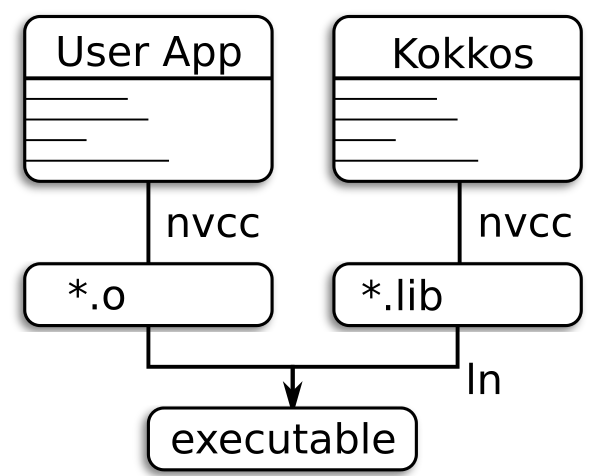
\includegraphics[width=0.3\textwidth]{img/Build.png}}
%\caption{The compilation workflow includes the invocation of the platform compiler that is in charge to generate parallel   Building workflow}
%\label{fig:workflow}  
%\end{figure}
